\documentclass[a4paper, 10pt]{article}

\usepackage[]{inputenc}
\usepackage{graphicx}
\usepackage[frenchb]{babel}
\usepackage{algorithm}
\usepackage{algpseudocode}
\usepackage{amsmath}
\usepackage{amsthm}
\usepackage{amsfonts}
\usepackage{dsfont }
\usepackage{wrapfig}
\usepackage[margin=1.4in]{geometry}
\begin{document}
	
	\title{Pattern Classification And Machine Learning : Project One, Group 16}
	\author{Marc Chachuat, Lie He, Alfonso Peterssen}
	\date{Due date : 31/10/2016} 
	
	\maketitle
	
	\section{Introduction}
	In this report, we explain the strategy we chosed to deal with this first project. This strategy can be divided in three parts answering to three questions : 
	\begin{enumerate}
		\item How to pre-process the data ? 
		\item How to train each model ? 
		\item How to choose the best model for the prediction? 
	\end{enumerate}
	In the following, a section is dedicated to each of these questions. 
	
	\section{Data pre-processing}
	
	Before even thinking to models and prediction, the first task of the data-scientist is to study his data and to pre-process them. The idea is essentially to remove the non relevant data, and to put the data set under a shape suitable for training the models.
	
		\subsection{Data cleaning}
		
		One of the first things we noticed in our training set, is that a lot of data were missing, replaced by $-999$ values. To avoid a bias, we decided to replace all the $-999$ values by the mean over the clean values of the current feature. Yet, after a lot of work we realized that this wasn't optimal, because some information was relying behind the fact that some features were missing for a given sample. \\
		
		\subsection{Feature Engineering}
		We decided to add a binary feature indicating whether or not at least one feature was originally missing for the given sample. This was concluding, as it increased our score.  Many features satisfy long tail distribution. These features are non-negative and are not centered near their mean. So we apply logarithm to them so that our learning algorithm will not be influenced too much by a few points. Besides, we convert feature 11 and 12 to categorical feature because they distributed like binary distribution. Additionally, Feature 22 is categorical and takes 4 values. We decompose them to 3 binary categorical features for better training results.
			
		We found that the training error of current model is large, meaning it is biased. To improve the performance, we need to enrich the model and by introducing more features with polynomial basis.  With the PCA we had reduced the dimension of each sample, which enabled us to make the label depends not only of the features, but also of power of the features. Then, another problem was to choose a suitable degree for polynomial basis. As a balance of performance and speed, we choose polynomial up to 3rd degree for non-crossed term ($x_1^2, ...$)  and 2nd degree for crossed term ($x_1x_2,...$)
		
		Finally, after the feature engineering, we rescale all the features to a similar level to have better convergence rate and prediction accuracy.
		
		\subsection{Selecting the relevant data}		
		The data set of the project contained a large number of features for each sample. This was a problem because it was considerably slowing our algorithm. Furthermore, we were suspecting that not all the data were relevant. We then had to select some. Yet, we hadn't the necessary background in physic to do it arbitrarily. We decided then to implement our own Principal Component Analysis. Running it on the training data set, it gives us a projector that projects all the data (validation, training and test sets) over a linear subspace of the data. Moreover, it enables us to choose the percentage of variance we wanted to keep.
		
	\section{Training of the models}
	
		As least squares method is a particular case of ridge regression, and logistic regression is a particular case of regularized logistic regression we decided to focus only on the ridge regression and on the regularized logistic regression.  For each of these models we had implemented training methods in the course. Yet, this was for a given lambda (regularization parameter) and a given degree for the polynomial basis. We realized then a grid search over a wide range of lambdas and degrees, training our models for each couple of parameters, and measuring its performance over the validation set. Finally, we kept for each model the couple of parameters ensuring the best performance. 
		
	\section{Choice of the model and prediction}

			
					\begin{figure}[!ht]
						\centering
						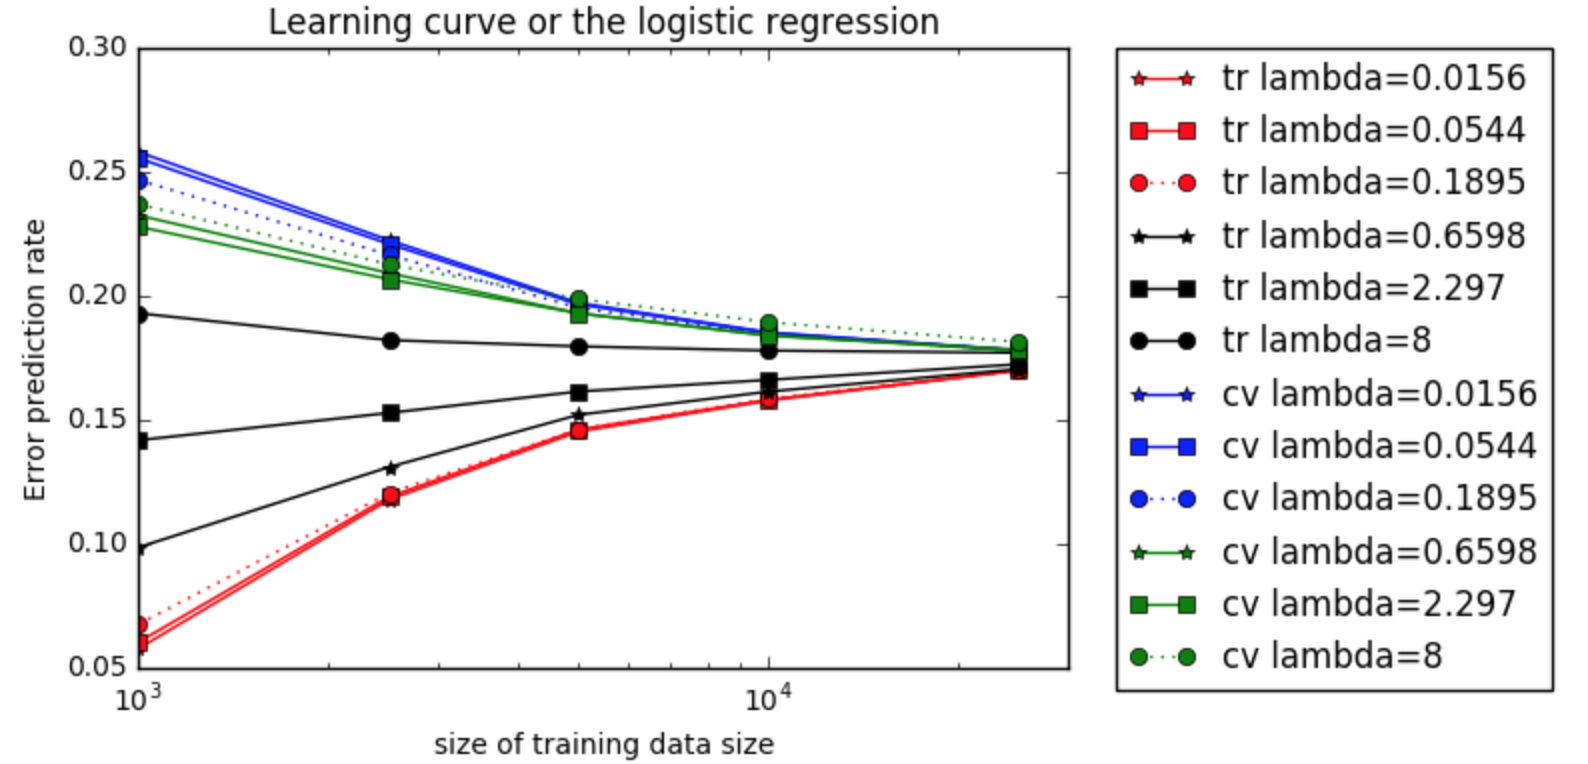
\includegraphics[width=0.5\textwidth]{fig}
						\caption{Learning Curve of Logistic regression with different regularization coefficients and training datasets}
						\label{fig:1}
					\end{figure}	

		In the above section, we mean by "performance", the accuracy over the validation set of the model trained over a training set. By using learning curve , we can find out if a training set size 
		is large enough to reduce overfitting and if a parameter is suitable for a model. In figure~\ref{fig:1}, the learning curve for logistic regression shows that it is reasonable to choose 28000 data points for training because the training error is close to cross validation error. We also find that the different choice of lambdas behave similarly for cross validation set, and thus choose $\lambda=0.5$ for or model. 
		
		Finally, to predict the labels for the submissions we just had to select the most performance of our two models by comparing the two optimal accuracy. The test accuracy will be over 82\% for this model, but in fact, we can have better performance by simply using higher order degree of polynomial of degrees and comparisons. The results of comparison are omitted here due to page limit.
\end{document}